\chapter{INFERENCE}

\renewcommand{\headrulewidth}{0.5pt}
\renewcommand{\footrulewidth}{0.5pt}
\thispagestyle{plain}
\pagestyle{fancy}
\fancyhf{}
\fancyhead[L]{\textbf{CHAPTER 4}}
\fancyhead[R]{\textbf{Intelligent Traffic System}}
\raggedright
\fancyfoot[L]{From: ITM Vision}
\fancyfoot[R]{Page \thepage}

\section{Optimization Methods}

    \subsection{Architecture Optimization}
        In the heterogeneous computing approach, the workload is divided between the processors with disparate architecture, viz. the CPU and GPU, to bring the best of two together. 
        Some works perform memory-level optimizations to GPU, such as using shared and texture memory, reducing accesses to global memory by using memory access coalescing and kernel fusion, etc. 
        Some works scale the frequency of CPU and/or GPU to tradeoff performance with energy. These works exploit slack in application deadlines or latency-tolerance of end-users to reduce frequency. 
        Many techniques exploit the error-tolerant nature of humans and neural network algorithms to trade off accuracy for achieving efficiency.
        \begin{itemize}
            \item At System and CPU-level, some optimization methods may be listed as CPU - GPU heterogeneous, pipelining, CPU frequency scaling, multithreading on CPU, etc
            \item At GPU-level, we can name a few such as: GPU frequency scaling, using TensorRT SDK, kernel fusion for reducing global memory transfer, executing kernels concurrently on different CUDA streams, 
            memory access coalescing, use CUDA managed memory, etc
            \item For approximate computing approaches, there are some examples as: using partial image instead of entire image, dropping unused rows in convolution, quantization, reducing bitwidth/precision, etc
        \end{itemize}

    \subsection{Algorithm Optimization}
        Algorithmic optimization methods come with a diversity as there are many works aims at improving efficiency of AI inference. A lot of works try to lowering image resolution, leverage knowledge distillation. 
        Some uses transfer learning, pointwise convolution, tucker decompositions or truncated singular value decomposition. The list is enlonged with CNN pruning and other matrix-related optimizations for such as: 
        converting matrix-vector product into matrix-matrix product, splitting matrix-multiplication in Fully Connected layer, matrix tiling, exploiting matrix sparsity. Some other optimizations may be count such 
        as merge batch normalization, loop unrolling, use of a-priori modules to remove most of the negative samples.

\section{TensorRT SDK}
    \subsection{Definition}
        NVIDIA \textregistered TensorRT \texttrademark is an SDK for high-performance deep learning inference. It includes a deep learning inference optimizer and runtime that delivers 
        low latency and high throughput for deep learning inference applications.
        \begin{figure}[H]
            \centering
            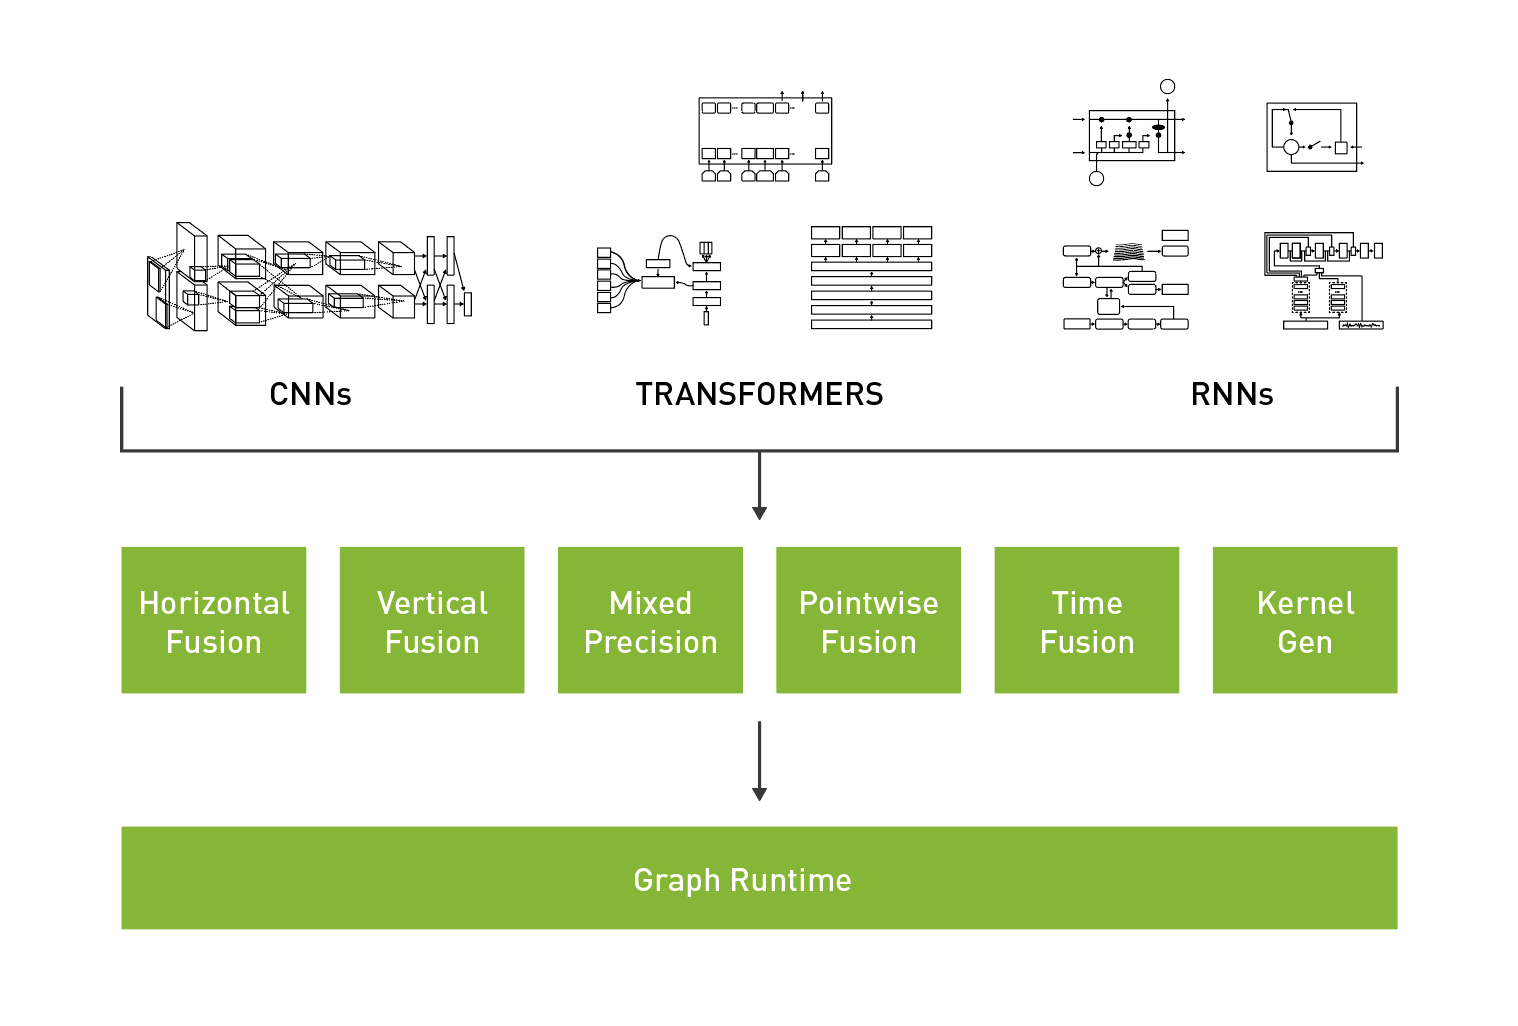
\includegraphics[width=0.6\linewidth]{img/tensorRt.png}
            \caption{TensorRT Pipeline}
        \end{figure}
        TensorRT-based applications perform up to 40X faster than CPU-only platforms during inference. With TensorRT, you can optimize neural network models trained in all major frameworks, 
        calibrate for lower precision with high accuracy, and deploy to hyperscale data centers, embedded, or automotive product platforms. \\ 
        \vspace{3mm}
        TensorRT is built on CUDA \textregistered, NVIDIA’s parallel programming model, and enables you to optimize inference leveraging libraries, development tools, and technologies in CUDA-X
        \texttrademark for artificial intelligence, autonomous machines, high-performance computing, and graphics. \\ 
        \vspace{3mm}
        TensorRT provides \textbf{INT8} and \textbf{FP16} optimizations for production deployments of deep learning inference applications such as video streaming, speech recognition, 
        recommendation, fraud detection, and natural language processing. Reduced precision inference significantly reduces application latency, which is a requirement for many real-time services, 
        as well as autonomous and embedded applications. \\ 
        \vspace{3mm}
        With TensorRT, developers can focus on creating novel AI-powered applications rather than performance tuning for inference deployment.
        \begin{figure}[H]
            \centering
            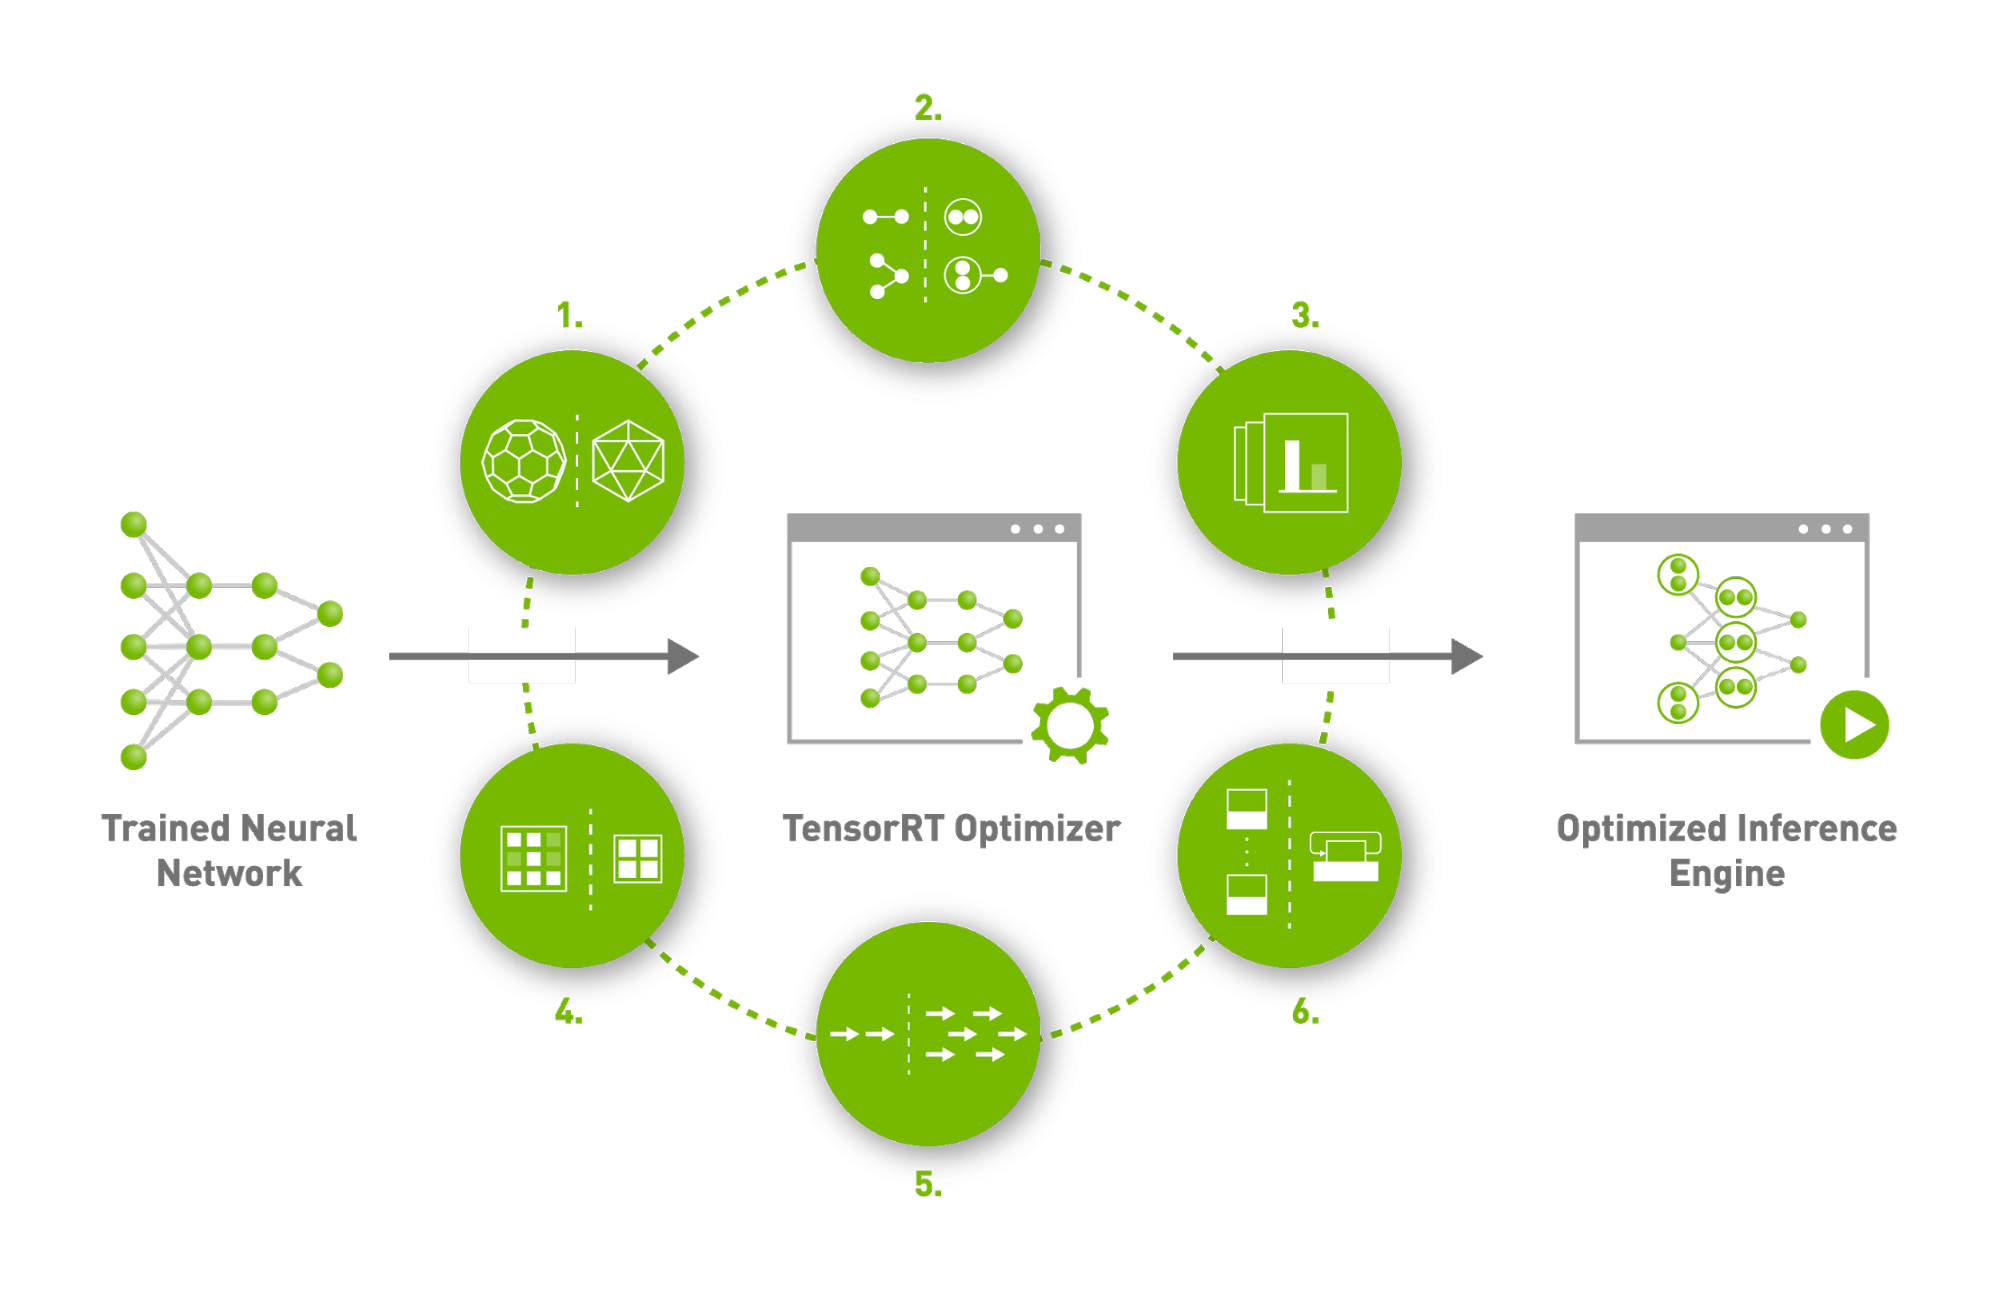
\includegraphics[width=0.6\linewidth]{img/inference-tensorrt.png}
            \caption{TensorRT Inference}
        \end{figure}
        \begin{enumerate}
            \item \textbf{Weight \& Activation Precision Calibration:} Maximizes throughput by quantizing models to \emph{INT8} while preserving accuracy.
            \item \textbf{Layer \& Tensor Fusion:} Optimizes use of GPU memory and bandwidth by fusing nodes in a kernel.
            \item \textbf{Kernel Auto-Tuning:} Selects best data layers and algorithms based on target GPU platform.
            \item \textbf{Dynamic Tensor Memory:} Minimizes memory footprint and re-uses memory for tensors efficiently.
            \item \textbf{Multi-Stream Execution:} Scalable design to process multiple input streams in parallel.
            \item \textbf{Time Fusion:} Optimizes recurrent neural networks over time steps with dynamically generated kernels.
        \end{enumerate}
    \subsection{What is TensorRT?}
        The core of NVIDIA \textregistered TensorRT \texttrademark is a C++ library that facilitates high-performance inference on NVIDIA graphics processing units (GPUs). 
        It is designed to work in a complementary fashion with training frameworks such as TensorFlow, Caffe, PyTorch, MXNet, etc. It focuses specifically on running an already-trained network quickly and 
        efficiently on a GPU for the purpose of generating a result (a process that is referred to in various places as scoring, detecting, regression, or inference). \\ 
        \vspace{3mm}
        Some training frameworks such as TensorFlow have integrated TensorRT so that it can be used to accelerate inference within the framework. Alternatively, TensorRT can be used as a library within a user application. 
        It includes parsers for importing existing models from Caffe, ONNX, or TensorFlow, and C++ and Python APIs for building models programmatically.
        \begin{figure}[H]
            \centering
            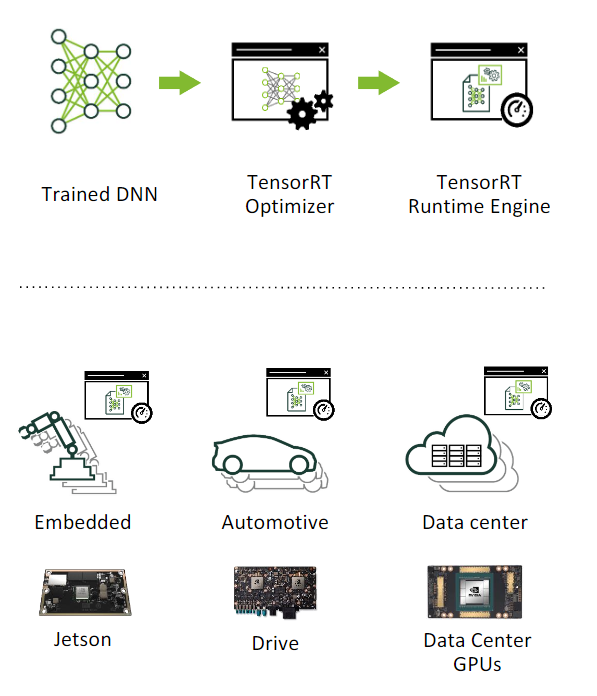
\includegraphics[width=0.6\linewidth]{img/high-performance.png}
            \caption{TensorRT defined as part high-performance inference optimizer and part runtime engine}
        \end{figure}
        TensorRT optimizes the network by combining layers and optimizing kernel selection for improved latency, throughput, power efficiency, and memory consumption. If the application specifies, 
        it will additionally optimize the network to run in lower precision, further increasing performance and reducing memory requirements.
        \begin{figure}[H]
            \centering
            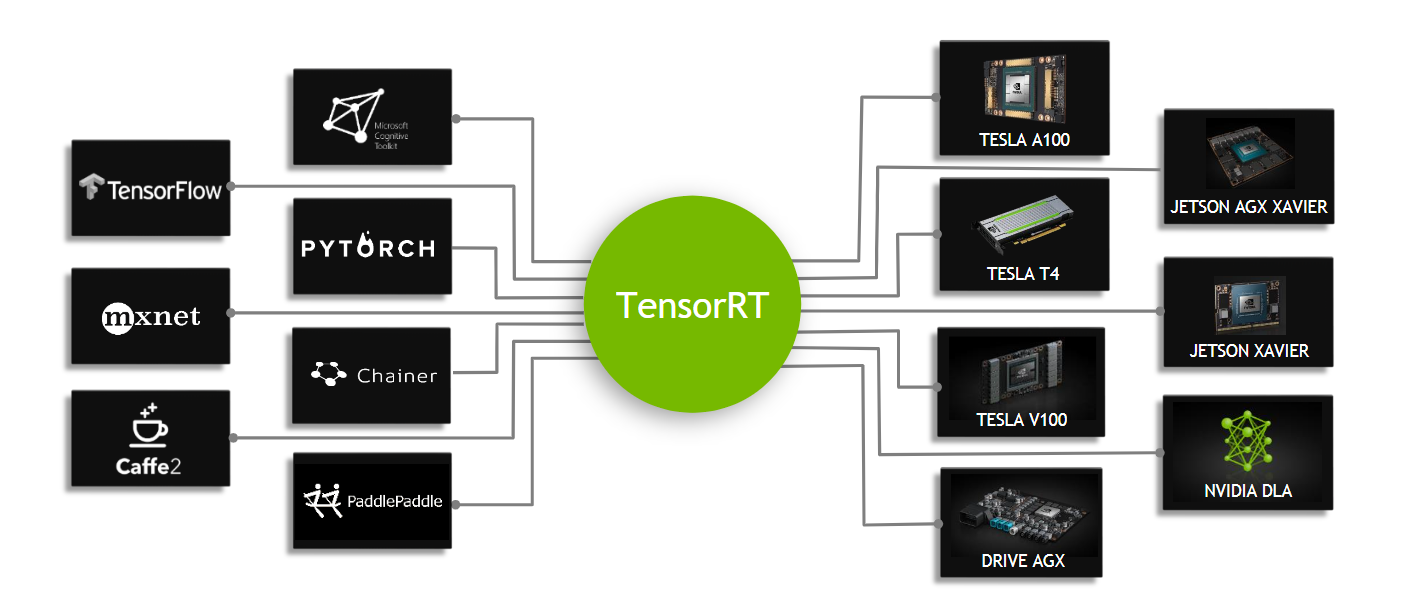
\includegraphics[width=0.6\linewidth]{img/application.png}
            \caption{TensorRT Application}
        \end{figure}
        The TensorRT API includes implementations for the most common deep learning layers. For more information about the layers, see TensorRT Layers. You can also use the \emph{C++ Plugin API} or \emph{Python Plugin API} 
        to provide implementations for infrequently used or more innovative layers that are not supported out-of-the-box by TensorRT. 
    \subsection{How does TensorRT work?}
        To optimize your model for inference, TensorRT takes your network definition, performs optimizations including platform-specific optimizations, and generates the inference engine. This process is referred to as the build phase. 
        The build phase can take considerable time, especially when running on embedded platforms. Therefore, a typical application will build an engine once, and then serialize it as a plan file for later use. \\ 
        \vspace{3mm}
        The build phase performs the following optimizations on the layer graph:
        \begin{itemize}
            \item Elimination of layers whose outputs are not used
            \item Elimination of operations which are equivalent to no-op
            \item The fusion of convolution, bias and ReLU operations
            \item Aggregation of operations with sufficiently similar parameters and the same source tensor (for example, the 1x1 convolutions in GoogleNet v5’s inception module)
            \item Merging of concatenation layers by directing layer outputs to the correct eventual destination.
        \end{itemize}
        The builder also modifies the precision of weights if necessary. When generating networks in 8-bit integer precision, it uses a process called calibration to determine the dynamic range of intermediate activations, 
        and hence the appropriate scaling factors for quantization. \\ 
        \vspace{3mm}
        In addition, the build phase also runs layers on dummy data to select the fastest from its kernel catalog and performs weight pre-formatting and memory optimization where appropriate.
    \subsection{What Capabilities Does TensorRT Provide?}
    TensorRT enables developers to import, calibrate, generate, and deploy optimized networks. Networks can be imported directly from Caffe, or from other frameworks via the UFF or ONNX formats. They may also be created programmatically by 
    instantiating individual layers and setting parameters and weights directly. \\ 
    \vspace{3mm}
    TensorRT provides a C++ implementation on all supported platforms, and a Python implementation on x86, aarch64, and ppc64le. \\ 
    \vspace{3mm}
    The key interfaces in the TensorRT core library are: \\ 
    \vspace{3mm}
    \ding{114} \textbf{Network Definition} \\ 
    \vspace{3mm}
    The Network Definition interface provides methods for the application to specify the definition of a network. Input and output tensors can be specified, layers can be added, and there is an interface for configuring each supported layer type. 
    As well as layer types, such as convolutional and recurrent layers, and a Plugin layer type allows the application to implement functionality not natively supported by TensorRT. \\ 
    \vspace{3mm}
    \ding{114} \textbf{Optimize Profile} \\ 
    \vspace{3mm}
    The Builder Configuration interface specifies details for creating an engine. It allows the application to specify optimization profiles, maximum workspace size, the minimum acceptable level of precision, timing iteration counts for autotuning, 
    and an interface for quantizing networks to run in 8-bit precision. \\ 
    \vspace{3mm}
    \ding{114} \textbf{Builder} \\ 
    \vspace{3mm}
    The Builder interface allows the creation of an optimized engine from a network definition and a builder configuration. \\ 
    \vspace{3mm}
    \ding{114} \textbf{Engine} \\ 
    \vspace{3mm}
    The Engine interface allows the application to execute inference. It supports synchronous and asynchronous execution, profiling, and enumeration and querying of the bindings for the engine inputs and outputs. A single-engine can have multiple execution contexts, 
    allowing a single set of trained parameters to be used for the simultaneous execution of multiple batches. \\ 
    \vspace{3mm}
    TensorRT provides parsers for importing trained networks to create network definitions: \textbf{Caffe Parser, UFF Parser, ONNX Parser.}


\section{Speed Estimation}
    \subsection{Mapping}
        To match track generated from pixel space to real space, we use perspective transform which projects a set of points from one 2D plane to another. 
        In this type of projection we are trying to approximate on a flat surface what is seen by the eye. This means usage of concepts such as vanishing 
        point convergence and the appearance of foreshortening, which means that an object's dimensions along the line of sight are shorter than its dimensions across the line of sight. \\ 
        \vspace{3mm}
        Perspective projection comes in several “flavors.” A one-point perspective contains only one vanishing point. A typical example is a set of train tracks. 
        If you stand on them and look into the distance, they converge to a single “vanishing point.” A two-point perspective has two vanishing points, 
        and a three-point has three vanishing points. Both of those  perspectives can be easily seen with sharp-angled buildings, and these perspectives are most often represented in outdoor scenes. \\ 
        \vspace{3mm}
        Here for ITS, all we have to do is provide the coordinates of four points — noncollinear, so defining the corners of a quadrilateral — in both coordinate systems. from these four points, 
        can translate a (u,v) pixel location to a (lon,lat) real world location, and vice versa. 
        \begin{figure}[H]
            \centering
            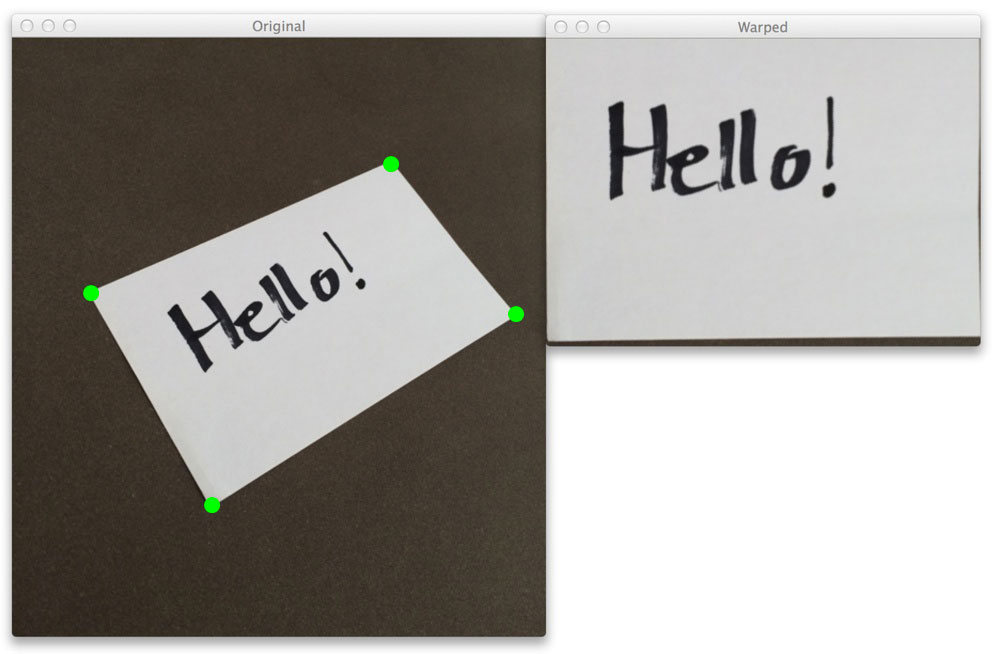
\includegraphics[width=0.6\linewidth]{img/perspective.png}
            \caption{Perspective Transformation}
        \end{figure}
        Applying this transformation to the (u,v) coordinates of our tracked objects, we can now plot their real world positions as they travel around the roundabout.
    \subsection{Speed Calculation}
        Using longgitude - latitudes we have just calculated, we perform another coordinate transform, this time converting the vehicle latitude-longitudes into a local Cartesian coordinate system, 
        with units in metres. This then allows us to easily calculate lengths and areas in these units. In order to calculate the vehicles’ speeds we need only to divide the distance — 
        calculated from the coordinates above — by the time.